%!TEX root = ../dissertation.tex

\chapter{Many-body localization}

\section{Locally boring globally exciting}
As we have seen in the previous chapter, isolated interacting many-body systems undergo thermalization dynamics when taken out of equilibrium. This causes the subsystem's degrees of freedom to be ultimately described by a thermal ensemble, even if the full system is in a pure \linebreak state~\cite{Deutsch1991, Srednicki1994, Rigol2008}. As a consequence, the local information about the initial state of the subsystem gets scrambled and transferred into non-local correlations that are only accessible through global \linebreak observables~\cite{Neill2016, Kaufman2016, Nandkishore2015}. 

Disordered systems can provide an exception to this paradigm of quantum thermalization. As was first pointed out by Anderson, in the presence of disorder the eigenstates of non-interacting particles exponentially localize\cite{Anderson1958}. This results in the long-term memory of the initial density distribution, which is at odds with the generic prediction for a subsystem to locally thermalize. This phenomenon has been observed on a number of different platforms \cite{Wiersma1997,  Schwartz2007, Billy2008, Roati2008, Lahini2008,Gadway2011, Kondov2011}. However, the question of whether thermalization survived in the disordered, interacting systems was more complicated and remained elusive.

Recent theoretical works have identified the presence of the localized phase in interacting systems which is called many-body localization (MBL) \cite{Nandkishore2015, Gornyi2005, Basko2006, Oganesyan2007, Imbrie2016, Altman2015, Abanin2018}. First experimental studies of interacting, disordered system were focused on the low laying part of the spectrum studying glassy dynamics \cite{DErrico2014, Kondov2015}. However, this phenomenon is qualitatively different from MBL as the latter describes the properties of the eigenstates of the system in the middle of the energy spectrum.  Later on, MBL has been experimentally probed through the persistence of the initial density distribution \cite{Schreiber2015, Smith2015, Bordia2016, Choi2016, Lueschen2017, Bordia2017}, demonstrating the breakdown of ergodicity in the system. 

While ergodicity breakdown is an important property of MBL, the presence of interaction in the system enables peculiar quantum many-body dynamics. Even for systems with only local interactions and in the absence of particle transport, non-local correlations are being generated during the dynamics.\cite{Znidaric2008, Bardarson2012}, which are inaccessible to local observables \cite{Serbyn2013, Serbyn2013a, Huse2014}. These dynamics are considered to be the hallmark of MBL and qualitatively distinguish it from its non-interacting counterpart, called Anderson localization \cite{Anderson1958, Schwartz2007, Billy2008, Roati2008, Lahini2008, Kondov2011, Jendrzejewski2012, Semeghini2015}. Experimental studies have observed a buildup of a two-point correlation function during transient dynamics \cite{Smith2015}, however, an unambiguous observation of non-local nature of correlations has remained elusive. Since the studies of this effect require exquisite control over the system's coherence for long evolution times.

\begin{figure*}[t]
	\centering
	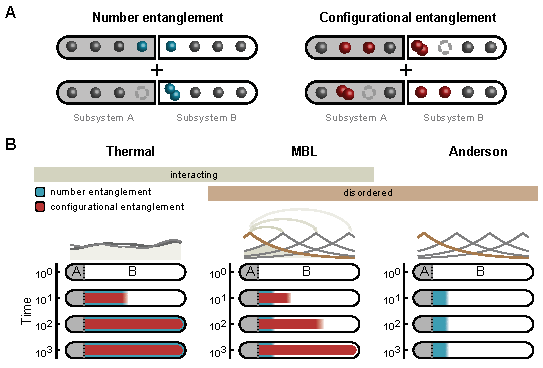
\includegraphics{figures/MBL_entropies.pdf}
	\caption{{\bf Entanglement dynamics in non-equilibrium quantum systems. (A)} Subsystems A and B of an isolated system out of equilibrium entangle in two different ways: \textit{number entanglement} is a superposition of states with different particle numbers in the subsystems and is generated through particle motion across the boundary; \textit{configurational entanglement} is a superposition of states with different particle arrangement within the subsystems and requires both particle motion and interactions. \textbf{(B)} In the absence of disorder, both types of entanglement rapidly spreads across the entire system due to delocalization of particles (left panel). The degree of entanglement and the timescales change drastically when applying disorder (central panel): particle localization spatially restrict number entanglement, yet interactions allow configurational entanglement to form very slowly across the entire system. A disordered system without interactions shows only local number entanglement while the slow growth of configurational entanglement is completely absent (right panel).}
	\label{fig:MBL_schematics}
\end{figure*}

We study these many-body dynamics by probing the entanglement properties of an MBL system with fixed total particle number \cite{ Znidaric2008, Bardarson2012, Serbyn2013, Serbyn2013a, Huse2014}. We distinguish two types of entanglement that can exist between a subsystem and its complement (see fig.~\ref{fig:MBL_schematics}~A): \textit{Number entanglement} implies that the particle number in one subsystem is correlated with the particle number in the other. It is generated by tunnelling across the boundary between the subsystems. \textit{Configurational entanglement} implies that the configuration of the particles in one subsystem is correlated with the configuration of the particles in the other. It arises from a combination of particle motion and interaction. The formation of particle and configurational entanglement changes in the presence or absence of interactions and disorder in the system (see fig.~\ref{fig:MBL_schematics}~B). In thermal systems without disorder, interacting particles delocalize and rapidly create both types of entanglement throughout the entire system. Contrarily, for Anderson localization, number entanglement builds up only locally at the boundary between the two subsystems. Here the lack of interactions prevents the substantial formation of configurational entanglement. In MBL systems, number entanglement builds up in a similarly local way as Anderson localization. However, notably, the presence of interactions additionally enables the slow formation of configurational entanglement throughout the entire system. 

\section{Disorder potential}

\begin{figure}[t]
	\centering
	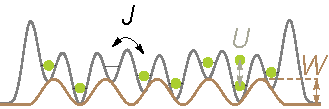
\includegraphics{figures/MBL_setup.pdf}
	\caption{\label{fig:MBL_model} \textbf{Experimental system.} We realize interacting Aubry-Andr\'e model, which is parametrized by the tunnelling rate $J/\hbar$, on-site interaction energy $U$ and quasi-periodic potential with amplitude $W$.}
\end{figure}

The properties of a system with “random on-site disorder” (especially a finite-size one) can be altered due to the presence of so called rare regions \cite{Agarwal2015, Agarwal2017, Roeck2017, Luitz2017, Nandkishore2017}, when neighboring sites can statistically have similar chemical potentials. In order to avoid this issue, we chose to study the system where disorder is given by periodic potential with incommensurate periodicity with respect to the lattice spacing. This realizes the interacting Aubry-Andr\'e model for bosons in one dimension \cite{Aubry1980, Iyer2013}, which is described by the Hamiltonian
\begin{equation}
\hat{\mathcal{H}} =  -J \sum_i \left(\hat{a}_i^\dagger\hat{a}_{i+1} + h.c.\right) 
+ \frac{U}{2} \sum_i\hat{n}_i \left( \hat{n}_i - 1\right) + W\sum_i h_i\hat{n}_i\text{,}
\end{equation}
where $\hat{a}_i^\dagger$ ($\hat{a}_i$) is the creation (annihilation) operator for a boson on site $i$, and $\hat{n}_i = \hat{a}_i^\dagger\hat{a}_i$ is the particle number operator on that site. The first term describes the tunneling between neighboring lattice sites with the rate $J/\hbar$, where $\hbar$ is the reduced Planck constant. The second term represents the energy shift $U$ when multiple particles occupy the same site. The last term introduces a site-resolved potential offset, which is created with an incommensurate lattice $h_i = \cos\left(2\pi\beta i+\phi\right)$ of period $\beta\approx 1.618$ lattice sites (which is a very good approximation for a golden ratio), phase $\phi$, and amplitude $W$. In our experiment, we achieve independent control over $J$, $W$, and $\phi$ (see fig.~\ref{fig:MBL_model}).

We use our DMD to project a disorder potential onto our atoms. A conceptually simple way of producing such a potential is to project a second lattice with incommensurate periodicity onto the bare lattice holding the atoms, e.g. by adding a potential of the form

\begin{equation}\label{eqn:Vsimple}
V_\text{simple}(x) = 2 \times W \cos^2\left(\pi\frac{x}{\beta a}+\phi\right)
\end{equation}

to the existing lattice. Since, $\beta$ is very close to the golden ratio $\beta-1 \approx \frac{1}{\beta}$, which means that, if the incommensurate potential is sampled when $x$ is integer multiples of $a$, any integer difference of $\beta$ results in the same sampled potential. 

\begin{figure}[t]
	\centering
	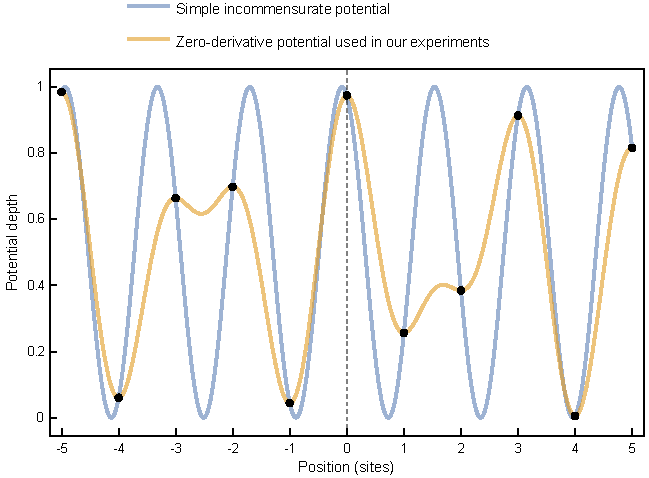
\includegraphics{figures/MBL_disorder.pdf}
	\caption{\label{fig:MBL_disorder} \textbf{Disorder engineering.} Plot showing a simple quasiperiodic disorder potential (blue) and the custom potential used in our experiments (yellow). The custom potential was engineered to yield the same on-site values as the simple one, but additionally possesses a vanishing first derivative at the position of the atoms (black dots), thereby making the system less sensitive to shaking-induced heating processes.}
\end{figure}


The potential in Eq.~\ref{eqn:Vsimple} has one major drawback: if the lattice site sits on the slope of the potential, the offset sampled by the atoms varies as the relative position of the disorder potential with respect to the bare lattice is perturbed, thereby making the system susceptible to shaking-induced heating processes. In order to make the system more robust, we set out to find a potential $V(x)$ that would provide the same on-site potential values as the potential in Eq.~\ref{eqn:Vsimple}, while also having a vanishing first derivative at the individual sites of the bare lattice, i.e. a potential $V(x)$ such that
$$ \left.V(x)\right\vert_{x = na} = \left.V_\text{simple}(x)\right\vert_{x = na} \hspace{1mm} , \hspace{1mm} \left. \frac{\partial V(x)}{\partial x} \right\vert_{x = na} = 0 \hspace{4mm} \forall \hspace{1mm} n \in \mathbb{Z} $$
where $a$ is the lattice constant of the bare lattice, and the position of an arbitrary lattice site is defined to be $x=0$. 

This can be achieved by using the property of the golden ration $\beta-1 = \frac{1}{\beta}$ and the fact that we only sample the potential at the integer points, resulting in:
\begin{equation}
cos^2\left(\pi\frac{x}{\beta a}\right) = cos^2\left(\pi\frac{(\beta -1)x}{ a}\right) = cos^2\left(\pi\frac{(\beta - m)x}{ a}\right),\hspace{4mm} \forall \hspace{1mm} x = n\cdot a
\end{equation}
for any pair of integers $m$  and $n$. One such potential is given by
\begin{equation}\label{eqn:Vapplied}
V_\text{dis}(x) =2 \times W\left [(2-\beta)\cos^2 \left(\pi(\beta-1)\frac{x}{a} + \phi \right) + (\beta-1)\cos^2 \left(\pi(\beta-2)\frac{x}{a} + \phi \right)\right ].
\end{equation}
Here both cosine functions have the same value at the position of the lattice sites as the original potential, and their amplitudes are chosen such that the derivative at the position of the sites is canceled. Figure \ref{fig:MBL_disorder} shows the potentials given by equations \ref{eqn:Vsimple} and \ref{eqn:Vapplied} in units of $W$ for $\phi = 0.16$.

\section{Calibration of the applied disorder potential}

\begin{figure}[htbp]
	\centering
	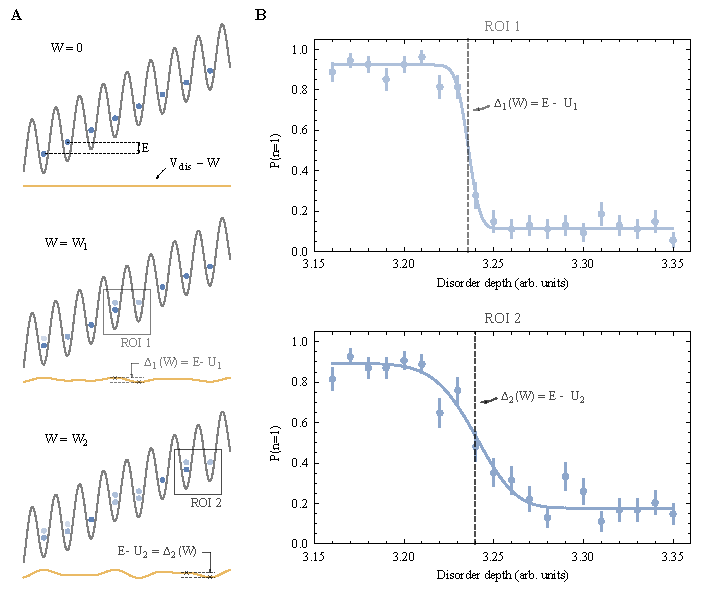
\includegraphics{figures/MBL_Wcal.pdf}
	\caption{\label{fig:Wcal} \textbf {Calibration of the disorder strength $W$ in our system.}  \textbf{(a)} We prepare the same tilted lattice system, where the tunneling is non-negligible but suppressed by the tilt. Afterwards, we adiabatically ramp the optical disorder power to different voltages on the corresponding photodiode and analyze the resulting number statistics for various regions of interest. If the disorder power $W$ is made sufficiently large, the potential difference $\Delta_i(W)$ it induces within a given region of interest may partially compensate for the linear tilt and enable resonant tunnelling processes (centre, bottom). \textbf{(b)} We again post-select on measurement outcomes with exactly two atoms in a given region of interest and plot the probability $P(n=1)$ of finding them on separate sites. The resulting curves show a sharp decay around the photodiode voltages where $\Delta_i(W) = E-U_i$, a condition allowing for resonant tunnelling processes that deplete the initial $n=1$ population.}
\end{figure}

In order to be able to compare our experimental results with numerical simulations, we need a precise knowledge of the exact chemical potential offsets experienced by the atoms. To measure that, we prepare an $n=1$ Mott insulator and turn on a magnetic field gradient along the direction of the chain, that offsets neighbouring sites by energy $E$. Subsequently, we change the lattice depth to an intermediate value where tunnelling is principally significant but still suppressed by the tilt. We adiabatically ramp up the power of the disorder potential to various values and image the atom number distribution along the chain (see fig.~\ref{fig:MBL_Wcal}a). When the potential difference between two neighbouring sites is equal to the applied tilt plus or minus $U$ (depending on which way the potential offsets the sites), one of the atoms is allowed to tunnel freely between the sites, resulting in the deviation from the uniform density. By plotting the post-selected unity-filling fraction for a given region $i$, we can identify the potential offset between any pair of sites in terms of $E$ and $U$, which we can calibrate independently in our system \cite{Ma2011} (see fig.~\ref{fig:MBL_Wcal}a).

In our experiment, we use $200$ different disorder patterns. Calibrating each one of them would be an extremely time-consuming procedure. However, since DMD should provide us with the exact Fourier transform of the displayed pattern, we can perform numerical Fourier transform of all used patterns and determine the potential difference between the sites for each one of them. In order to verify that the potentials experienced be the atoms do not suffer from the aberrations of the imaging system and other possible imperfections, we measure all potential differences within one pattern and compare them to the result of the Fourier transform (see fig.~\ref{fig:MBL_Wcal}). Excellent agreement of the measurement with numerical Fourier transform indicates the applicability of our method.

\begin{figure}[t]
	\centering
	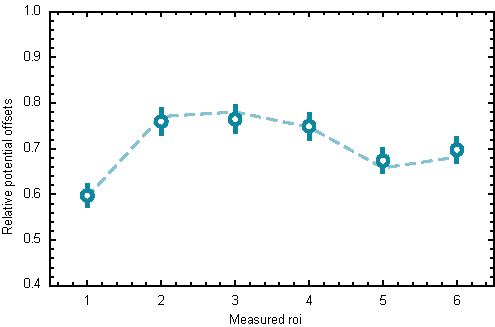
\includegraphics{figures/MBL_disorder_cal_roi.pdf}
	\caption{\label{fig:MBL_Wcal} \textbf {Relative potential offsets within one pattern.} In order to benchmark the applied disorder potential, we compare the measured site offsets within one pattern to the numerical Fourier transform of the corresponding hologram (dotted line). The agreement between the data and numerical prediction confirms the high level of control over the applied optical potential. The relative potential offsets (both data and numerical prediction) are normalized to the largest potential difference in all applied patterns.}
\end{figure}

Our numerical studies show, that the exact potential differences do not exactly coincide with true quasi-periodic lattice potential (see fig.~\ref{fig:MBL_potential}). For all numerical simulations in this chapter, we use the disorder values extracted from the Fourier transforms of the holograms.

\begin{figure}[t]
	\centering
	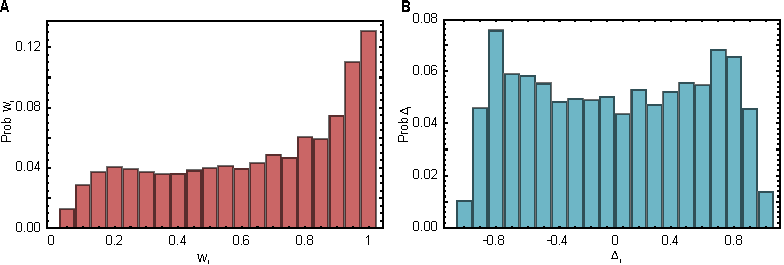
\includegraphics[width=140mm]{figures/MBL_dists_combo.pdf}
	\caption{\label{fig:DistRow} {\bf Distribution of the disorder potential.}  The left plot is a histogram of the DMD generated on-site quasi-periodic potential ($W_i$) which is normalized to $1$. The right plot is a histogram of the inter-site difference of the DMD generated quasi-periodic potential ($\Delta_i$)}.
	\label{fig:MBL_potential}
\end{figure}

\section{Breakdown of thermalization}

In order to investigate the breakdown of thermalization, we focus on the subsystem that consists of a single lattice site. The conserved total atom number enforces a one-to-one correspondence between the particle number outcome on a single site and the number in the remainder of the system---entangling the two during tunnelling dynamics. Ignoring information about the remaining system puts the subsystem into a mixed state of different number states. The associated number entropy is given by $S_\text{n}^{(1)} = -\sum_{n} p_n \log(p_n)$, where $p_n$ is the probability of finding $n$ atoms in the subsystem. Since the atom number is the only degree of freedom of a single lattice site, $S_\text{n}^{(1)}$ captures all of the entanglement between the subsystem and its complement and is equivalent to the single-site von Neumann entanglement entropy $S_\text{vN}^{(1)}$.

\begin{figure}[t]
	\centering
	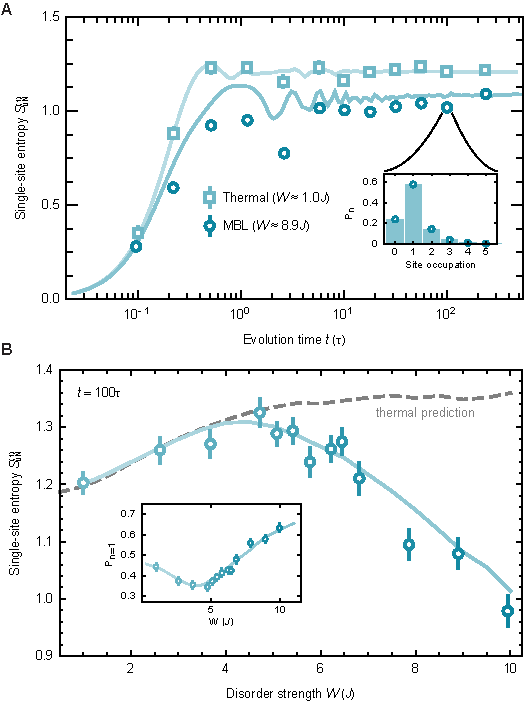
\includegraphics[width=\textwidth]{figures/MBL_ETH_breakdown.pdf}
	{\caption{{\bf Breakdown of thermalization on a single site level (A)} We compute the single-site von Neumann entropy $S_\text{vN}^{(1)}$ from the site-resolved atom number statistics (inset) after different evolution times (scaled with tunneling time $\tau=\hbar/J$) in the presence of weak and strong disorder. {\bf(B)} Probability $p_1$ to retrieve the initial state (inset) and $S_\text{vN}^{(1)}$ for different $W$, measured after $100\tau$ evolution. The deviation from the thermal ensemble prediction for strong disorder signals the breakdown of thermalization in the system. All solid lines show the prediction of exact diagonalization calculations without any free parameters. Each data point is sampled from 197 disorder realizations (see Appendix~\ref{AppendixB}). Error bars denote the s.e.m.}
	\label{fig:MBL_ETH_breakdown}}
\end{figure}

Counting the atom number on an individual lattice site in different experimental realizations allows us to obtain the probabilities $p_n$ and compute $S_\text{vN}^{(1)}$. We perform such measurements for various evolution times. At low disorder depth ($W=1.0(1)J$), the entropy grows over a few tunnelling times and then reaches a stationary value (see fig,~\ref{fig:MBL_ETH_breakdown}~A). The stationary value is reduced for a deep disorder ($W=8.9(1)J$) and remains constant over two orders of magnitude in evolution time, up to several hundred tunnelling times. The lack of entropy increase indicates the absence of heating in the system. The excellent agreement of the measured entropy with \textit{ab initio} calculations up to the longest measured evolution times suggests a highly unitary evolution of the system.

We perform measurements of $S_\text{vN}^{(1)}$ at different disorder strengths following an evolution of one hundred tunneling times (see fig,~\ref{fig:MBL_ETH_breakdown}~B). To evaluate the degree of local thermalization, we compare the results with the prediction of a thermal micro-canonical ensemble for our system. For weak disorder, the measured entropy agrees with the predicted value, whereas the entropy is significantly reduced for strong disorder--- signalling the absence of thermalization in the system. As a consequence, the system retains some memory of its initial conditions for arbitrarily long evolution times. We indeed find that the probability to retrieve the initial state of one atom per site increases for the strong disorder (see fig,~\ref{fig:MBL_ETH_breakdown}~B).

The thermal prediction, shown in the figure~\ref{fig:MBL_ETH_breakdown}~B is calculated using a microcanoical ensemble: equal probabilities statistical mixture of 11 eigenstates of the evolution Hamiltonian $H_{evo}(W)$, that are closest to the average energy of the initial state, given by $E_0=\bra{\psi_0}H_{evo}(W)\ket{\psi_0}$. We verify that the results do not depend on the exact number of included eigenstates in the vicinity of the chosen value.  

\section{Spatial localization}

The breakdown of thermalization is expected to be a consequence of the spatial localization of the particles. Previous experiments have determined the decay length of an initially prepared density step into empty space \cite{Choi2016}. We measure the localization by directly probing density-density correlations within the system. These correlations are captured by $G^{(2)}(d)=\langle n_{i} n_{i+d} \rangle - \langle n_{i}\rangle \langle n_{i+d}\rangle$, where $\langle...\rangle$ denotes averaging over different disorder realizations as well as all sites $i$ of the chain. The particle numbers on two sites at distance $d>0$ are uncorrelated for $G^{(2)}(d)=0$. If a particle moves a distance $d$, the sites become anti-correlated, and the correlator decreases to $G^{(2)}(d)<0$. 

\begin{figure}[t]
	\centering
	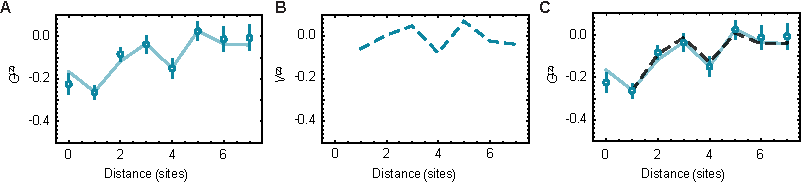
\includegraphics[width=140mm]{figures/MBL_G2Combo_Row.pdf}
	\caption{\label{fig:MBL_g2} \textbf{Potential and Wavefunction: Two-Point Correlations. } The left plot shows the measured $G_2(r)$ data for an 8 site, 8 atom system after 100 tunneling times with disorder strength $W=5.8J$ and $U=2.7J$. This solid line is from simulation performed by exact diagonalization for the same experimental parameters. The middle plot is the calculated two-point correlator for the applied quasi-periodic potential and averaged over may different disorder realizations -- the qualitative features in the left plot mimic the correlation function of the applied potential.The right plot is the same data with the fitted correlation function (black) made from the applied potential correlations ansatz (eq. \ref{eqn:g2fit}).}
\end{figure}
For a moderate disorder strength, we observe, that the measured correlation function has some structure in it (see fig.~\ref{fig:MBL_g2}~A). This can be explained by taking into account the correlations that are inherent to the disorder potential itself. Consider $V(x,\phi) = \cos{\left ( 2 \pi \beta x + \phi \right ) }$, we can define two-point correlation function of the potential as
\begin{equation}\label{eqn:v2}
V_{2}(d)= \langle V(x,\phi) V(x+d,\phi) \rangle_{d,\phi} -  \langle V(x,\phi)  \rangle_{d,\phi}  \langle V(x+d,\phi) \rangle_{d,\phi} ,
\end{equation}
where $\phi$ runs over all possible phases of the disorder (see fig.~\ref{fig:MBL_g2}~B). In order to unbias our results from the effects coming from the potential, we introduce a fitting ansatz, that takes into account the correlations of the potential
\begin{equation}\label{eqn:g2fit}
G_{2}^{fit}(d)= (A+B \times  V_2(d)) e^{-d/\xi},
\end{equation}
where $A$, $B$, and $\xi$ are fitting parameters. Subtracting those effects leads to $\widetilde{G^2}(d) = G^{(2)}(d) - B \times  V_2(d) e^{-d/\xi}$, that we use to interpret our results.

\begin{figure}[t]
	\centering
	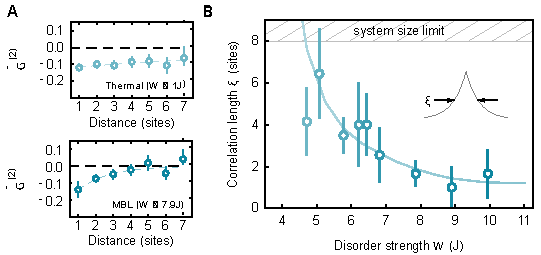
\includegraphics{figures/MBL_localization.pdf}
	\caption{{\bf Spatial localization of the particles.} {\bf{(A)}} The density-density correlations $\widetilde{G^{2}}(d)$ as a function of distance $d$ at weak and strong disorder after an evolution time of $100\tau$. {\bf (B)} Particle motion is confined within the correlation length $\xi$. We use a fit to extract $\xi$ for different disorder strengths. The fit function is a product of an exponential decay with the autocorrelation function of the quasiperiodic potential. Each measurement is sampled from 197 disorder realizations. The solid lines show the prediction of exact diagonalization---calculated without any free parameters. Error bars denote the s.e.m in {\bf (A)}, and the fit error in {\bf (C)}.}
	\label{fig:MBL_localization}
\end{figure}

We measure the density-density correlations $\widetilde{G^{2}}(d)$ for different disorder strengths in the stationary regime (see fig.~\ref{fig:MBL_localization}). For low disorder, we find the correlations to be independent of distance and below zero. This indicates that the particles tunnel across the entire system and hence are delocalized. On the other hand, at the strong disorder, only nearby sites show significant correlations, signalling the absence of particle motion across large distances. We thus conclude that the particles are localized. We extract the correlation length by fitting an exponentially decaying function to the data (see fig.~\ref{fig:MBL_localization}~A). For increasing disorder, the correlation length decreases from the entire system size down to around one lattice site (see fig.~\ref{fig:MBL_localization}~B). 

Our observation of localized particles is consistent with the description of MBL in terms of local integrals of motion \cite{Serbyn2013, Serbyn2013a, Huse2014}. It describes the global eigenstates as product states of exponentially localized orbitals. The correlation length extracted from our data is a measure of the size of these orbitals. Since the latter form a complete set of locally conserved quantities, this picture connects the breakdown of thermalization in MBL with non-thermalizing, integrable systems. 

\section{Different types of entanglement}

We now turn to a characterization of the entanglement properties of larger subsystems, starting with a subsystem covering half the system size. As for the case of a single lattice site, the particle number in the subsystem can become entangled with the number in the remaining system through tunnelling dynamics. However, subsystems which extend over several lattice sites, with a given particle number, offer the particle configuration as an additional degree of freedom for the entanglement. 

In the Schmidt basis the density matrix for the subsystem $\rho$ has only diagonal elements, and the von Neumann entropy can be written as
\begin{equation}
S_\text{vN}=\sum_i \rho_{ii} \log {\left ( \rho_{ii} \right )}.
\end{equation}
If the global particle number is conserved, there can not be any coherence between the states with different particle number
within the subsystem, since the particle number in the subsystem's complement is uniquely determined. Therefore  the density matrix can be written as $\rho_{ii} = p_n \rho_{ii}^{(n)}$, where $p_n = \sum_{ii \subset n} \rho_{ii}$ is the probability of having $n$ particles within the subsystem and $\rho_{ii}^{(n)}$ describe the relative probability of being in the certain state within the given particle number sub-sector, such that $\sum_{ii} \rho_{ii}^{(n)}=1$. Hence the von Neumann entropy can be written as:

\begin{equation}
\begin{aligned}
S_\text{vN}=&\sum_{n=0}^N \sum_i p_n  \rho_{ii}^{(n)} \log {\left (p_n \rho_{ii}^{(n)} \right )}=\sum_{n=0}^N \sum_i p_n  \rho_{ii}^{(n)} \left (\log{\left ( p_n \right )} + \log {\left ( \rho_{ii}^{(n)} \right )} \right ) = \\
&=\sum_{n=0}^N p_n  \log{\left ( p_n \right )}  \sum_i \rho_{ii}^{(n)} + \sum_{n=0}^N p_n \sum_{i} \rho_{ii}^{(n)} \log {\left ( \rho_{ii}^{(n)} \right )} = \\
&=\sum_{n=0}^N p_n  \log{\left ( p_n \right )}  + \sum_{n=0}^N p_n \sum_{i} \rho_{ii}^{(n)} \log {\left ( \rho_{ii}^{(n)} \right )}=\\
&=S_\text{n} + S_\text{c}
\end{aligned}
\end{equation}

The first term:
\begin{equation}
S_\text{n} = \sum_{n=0}^N p_n  \log{\left ( p_n \right )},
\end{equation}
we call number entanglement, describes how many sub-sectors with different particle number in the subsystem are populated. This entanglement is created through particle tunneling between two subsystems. The second term:
\begin{equation}
S_\text{c} = \sum_{n=0}^N p_n \sum_{i} \rho_{ii}^{(n)} \log {\left ( \rho_{ii}^{(n)} \right )},
\end{equation}
we call configurational entanglement. It measures how many states within the same sub-sector are occupied. This type of entanglement only builds up substantially in interacting systems, since configurational correlations require an arrangement of several particles in the different subsystems. An analogous split can be done of any conserved quantity and for example also exists for spin systems with conserved total magnetization instead of the particle number. 

\section{MBL as a system of local integrals of motion}

The universal properties of entanglement dynamics in the MBL phase could be understood from the phenomenological model\cite{Serbyn2013, Serbyn2013a, Huse2014}. It states that eigenstates of an MBL system can be decomposed into a product state of local integrals of motion, that we refer to as localized orbitals. Although their exact structure in terms of original particle operators can be quiet complicated\cite{Serbyn2013a}, the knowledge of exact mapping is not necessary in order to understand the resulting dynamics. 

Each of those orbitals can be in an arbitrary superposition of different occupation states, determined by the initial state projection. Furthermore, the combination of original particles tunnelling and interactions result in the  effective Hamiltonian for the localized orbitals:
\begin{equation}
\hat{\mathcal{H}} = U_{eff}\sum_{i,j} e^{-\left| i-j\right|/\xi}\hat{o_i}\hat{o_j},
\end{equation}
where $\hat{o_i}$ is the occupation number operator the localized orbital $i$ and $U_{eff}$ is a constant given by the parameters of the original system. The exponential decay of interactions strength is due to the localized nature of the orbitals and $\xi$ is their effective localization length.

In order to understand the dynamics of the system under this model, let's consider a simple example of two orbitals $i$ and $j$. As we mentioned before and as the form of the Hamiltonian suggests, the occupation number of each of the orbitals in a conserved quantity. First, notice that the only effect the time evolution has on the pair of orbital $i$ and $j$ is to advance the phase between different occupation states of one of them depending on the state of the other. Second, if the orbitals start in the single occupational state the time evolution has a trivial effect of overall phase accumulation and, hence, can not lead to the entanglement between the orbitals.

However, if both orbitals start in the superposition of different occupation states, the system's dynamics will produce entanglement between the two at certain time points. To see that, consider an initially unentangled state 
\begin{equation}
\ket{\psi(0)} = (\ket{0}+\ket{1})\otimes(\ket{0}+\ket{1}) = \ket{00}+\ket{01}+\ket{10}+\ket{11}.
\end{equation}
Under the time evolution only the last term has non-trivial dynamics, such that after a time $t$ the state reads
\begin{equation}
\ket{\psi(t)} = \ket{00}+\ket{01}+\ket{10}+e^{iU_{eff}t/\hbar}\ket{11},
\end{equation}
and after $t_{ent}=\pi \frac{\hbar}{U_{eff}}$ we get
\begin{equation}
\ket{\psi(t_{ent})} = \ket{00}+\ket{01}+\ket{10}-\ket{11} = \ket{0}\otimes(\ket{0}+\ket{1})+\ket{1}\otimes(\ket{0} -\ket{1}).
\end{equation}
The final state is maximally entangled, since two states of each orbital are orthogonal to each other. Note, that this effect is purely quantum, since it stems form the coherent phase evolution of the superposition states, hence it can not be captured by any mean-field approach or classically interacting particles.

\begin{figure}[t]
	\centering
	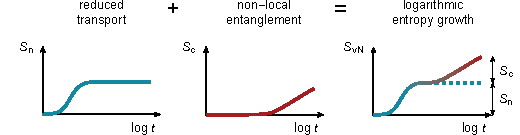
\includegraphics[scale=1.6]{figures/MBL_ent_split.pdf}
	\caption{{\bf Entropy dynamics in MBL.} The von-Neumann entanglement entropy is the sum of the number entropy and the configurational entropy, whose dynamics in an MBL system occur over different time scales.}
	\label{fig:MBL_ent_concept}
\end{figure}

The dynamics of $S_\text{n}$ and $S_\text{c}$ in the MBL regime \ref{fig:MBL_ent_concept} can be understood in the picture of localized orbitals. Since the localized orbitals restrict the particle motion, the number entropy can only develop within the localization length and hence $S_\text{n}$ saturates at a lower value than for the thermal case. In the MBL regime, disorder suppresses the tunnelling. Therefore, saturation is reached at a later time. However, the dynamics of $S_\text{c}$ are strikingly different, as they are governed by the relative phase evolution between different many-body states.  The effective interactions among the orbitals decay exponentially with the distance between them. As a consequence, entanglement between distant orbitals forms slowly, causing a logarithmic growth of $S_\text{c}$, even after $S_\text{n}$ has saturated \cite{Serbyn2013, Serbyn2013a, Huse2014, Znidaric2008, Bardarson2012}.

\section{Accessing configurational entanglement through correlations}
In our experiment, we can independently probe both types of entanglement. We obtain the number entropy $S_\text{n}$ through the probabilities $p_n$ by counting the atom number in the subsystem in different experimental realizations. The configurational entropy $S_\text{c}$, in contrast, is challenging to measure in a many-body system since it requires experimental access to the coherences between a large number of quantum states \cite{Islam2015, Elben2017}. Here we choose a complementary approach to probe the configurational entanglement in the system. It exploits the configurational correlations between the subsystems, quantified by the correlator:
\begin{equation}
C = \sum_{n=0}^{N}p_n \sum_{\{A_{n}\},\{B_{n}\}}\left| p(A_{n} \otimes B_{n}) - p(A_{n}) p(B_{n}) \right| ,
\end{equation}
where $\{A_{n}\}$ ($\{B_{n}\}$) is the set of all possible configurations of $n$ particles in subsystem A ($N-n$ in B), and $N$ is total number of particles in the system. All probability distributions are normalized within the subspaces of $n$ particles in A and the remaining $N-n$ particles in B. The configuration $A_{n} \otimes B_{n}$ is separable if $p(A_{n} \otimes B_{n}) = p(A_{n}) p(B_{n})$. The correlator therefore probes the entanglement through the deviation from separability between A and B. 

In general, one does not a priory expect that there should be any linear relation between $S_c$ and and $C$. In fact, their asymptotic behavior is very different from one another. While $S_c$ is a unbounded quantity, the correlator $C$ has an upper bound of $2$. To see that
\begin{equation}
\begin{aligned}
&C = \sum_{n=0}^{N}p_n \sum_{\{A_{n}\},\{B_{n}\}}\left| p(A_{n} \otimes B_{n}) - p(A_{n}) p(B_{n}) \right| \leq \\
&\leq  \sum_{n=0}^{N}p_n \sum_{\{A_{n}\},\{B_{n}\}}\left| p(A_{n} \otimes B_{n})\right| + \left| p(A_{n}) p(B_{n}) \right|  = 2 \sum_{n=0}^{N}p_n  = 2.
\end{aligned}
\end{equation}
However, in the localized regime for sufficiently small amounts of entanglement, our numerical studies show, that the two are proportional to one another (see fig.~\ref{fig:MBL_c_Sc}). This proportionality even hold for different values of intercalation strength, making it a good proxi for configurational entropy in such systems.
\begin{figure}[t]
	\centering
	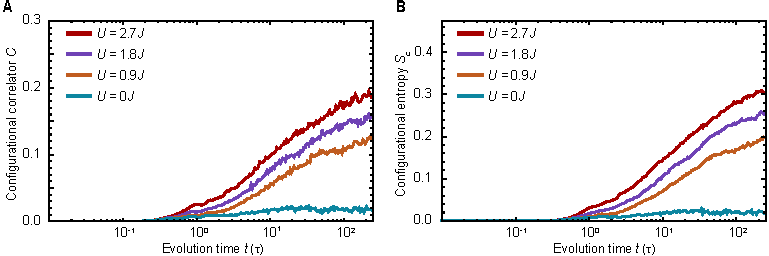
\includegraphics{figures/MBL_C_SC.pdf}
	\caption{\label{fig:MBL_c_Sc} \textbf{Correlations and Configurational Entropy.} {\bf (A)} The configurational correlations  as measured in the Fock basis is plotted as a function of interaction strength and evolution time. {\bf (B)} The corresponding configurational entropy is plotted in the right as a function of interaction strength and evolution time.  All of these simulations were performed by exact diagonalization on 6 sites with 6 atoms.}
\end{figure}

As pointed out in \cite{Nanduri2014}, the total amount of entanglement in the MBL phase depends on the initial state of the system. Therefore, for any system size, the maximal amount of entanglement can be adjusted such that the proportionality between $S_C$ and $C$ holds for the entire duration of time evolution, making the correlator a very powerful tool to study this phenomenon. The correlator $C$ is also experimentally more accessible than $S_c$, since it involves projective measurements in the particle number basis. Therefore, it can be generalized to higher dimensions and different experimental platforms, e.g. trapped ions, neutral atoms, superconducting circuits, where a direct measurement of entanglement entropy remains challenging.

\begin{figure}[t!]
	\centering
	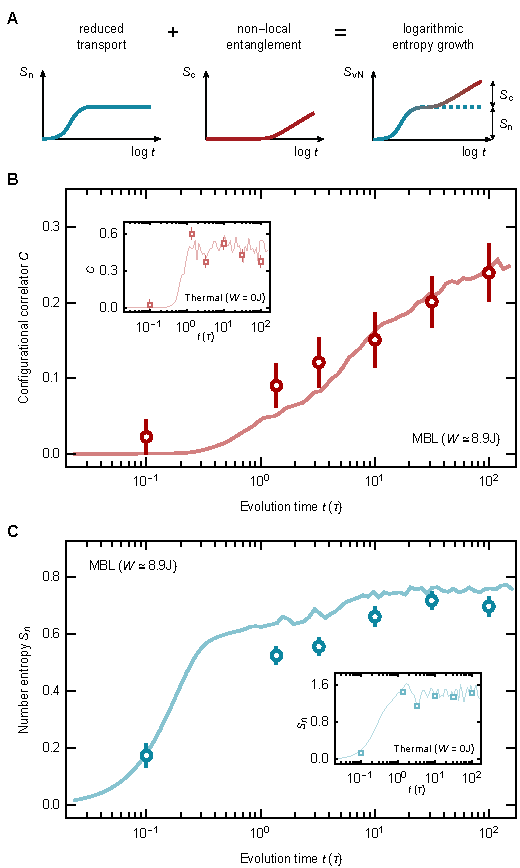
\includegraphics{figures/MBL_entropy_dynamics.pdf}
	\caption{{\bf Dynamics of the number and configurational entanglement. } {\bf (A)} We probe the configurational entropy with the correlator $C$. At strong disorder, it shows a persistent slow increase that is consistent with a logarithmic growth in time, until the longest evolution times covered by our measurements. {\bf (B)} The number entropy $S_\text{n}$ reaches a stationary value within few tunneling times. Without disorder, the entanglement dynamics change: both $S_\text{n}$ and $C$ quickly reach a stationary value (insets). The solid lines show the prediction of exact diagonalization calculations without any free parameters. The above data was taken on a six-site system and averaged over four disorder realizations. Error bars denote the s.e.m.}\label{fig:MBL_entropy_dynamics}
\end{figure}

\section{Entropy dynamics and scaling}

We study the time dynamics of $S_\text{n}$ and $C$ with and without disorder (see fig.~\ref{fig:MBL_entropy_dynamics}). Without disorder, both $S_\text{n}$ and $C$ rapidly rise and reach a stationary value within a few tunnelling times (insets). In the presence of strong disorder, we find a qualitatively different behaviour for the two quantities: $S_\text{n}$ reaches a stationary state within few tunnelling times, although after longer evolution time due to reduced effective tunnelling. Additionally, the stationary value is significantly reduced, indicating suppressed particle transport through the system. The correlator $C$, in contrast, shows a persistent slow growth up to the longest evolution times reached by our measurements. The growth is consistent with logarithmic behaviour over two decades of time evolution. We conclude that we observe interaction-induced dynamics in the MBL regime, which are consistent with the phenomenological model \cite{Serbyn2013, Serbyn2013a, Huse2014}. The agreement of the long-term dynamics of $S_\text{p}$ and $C$ with the numerical calculations in the MBL regime confirms the unitary evolution of the system within its 6435-dimensional Hilbert space over $100\,\tau$. The system remains in the finite-time limit, not in the finite-size limit since the spread of entanglement has not yet stopped at the longest studied evolution times. 

Considering the entropy in subsystems of different size gives us insights into the spatial distribution of entanglement in the system: in a one-dimensional system, locally generated entanglement results in a subsystem size independent entropy, whereas entanglement from non-local correlations causes the entropy to increase in proportion to the size of the subsystem. In reference to the subsystem's boundary and volume, these scalings are called area law and volume law. We find almost no change in $S_\text{n}$ for different subsystems of an MBL system (see fig.~\ref{fig:MBL_scalings}~A)---indicating an area law scaling due to localized particles and confirming that particle transport is suppressed. In contrast, the configurational correlations $C$ increase until the subsystem reaches half the system size (see fig.~\ref{fig:MBL_scalings}~B). Such a volume-law scaling is also expected for the entanglement entropy and demonstrates that the observed logarithmic growth indeed stems from non-local correlations across the entire system.

\begin{figure}[t]
	\centering
	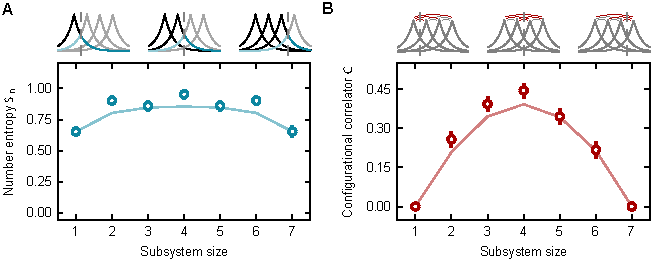
\includegraphics{figures/MBL_scaling.pdf}
	\caption{{\bf Spatial distribution of the entanglement.} Number entropy and configurational correlator in the MBL regime ($W=8.9\,J$) after an evolution time of $100\tau$. {\bf (A)} The number entropy $S_\text{n}$ does not depend on the subsystem size, i.e. follows an area law. {\bf (B)} The configurational correlator $C$ increases almost linearly with the subsystem size, showing a volume-law behavior. The solid lines show the prediction of exact diagonalization calculations without any free parameters. The above data was averaged over four disorder realizations. Error bars denote the s.e.m. and are below the marker size if hidden.}
	\label{fig:MBL_scalings}
\end{figure}

\section{Conclusion}

Investigating the growth of non-local quantum correlations has been a long-standing experimental challenge for the study of MBL systems. In addition to achieving exceptional isolation from the environment and local access to the system, such a measurement requires access to the entanglement entropy \cite{Islam2015}. Our work provides a novel method to characterize the entanglement properties of MBL systems. Since it is based on measurements of the particle number fluctuations and their configurations, the method is experimentally accessible and can be generalized to higher dimensions and different experimental platforms, where direct measurement of entanglement entropy remains challenging, e.g. trapped ions, neutral atoms, superconducting qubits. The observation of slow coherent many-body dynamics along with the breakdown of thermalization coincides with the expected behaviour for larger systems and allows us to unambiguously identify and characterize the MBL state in our system.

In future, experiments at different system sizes will be of interest to shed light on the critical properties of the thermal-to-MBL phase transition, which are the subject of ongoing studies \cite{Vosk2015, Potter2015, Khemani2017, Lueschen2017a}. In our system, it is experimentally feasible to continue scaling the system size at unity filling to a numerically intractable regime. Additionally, we have full control over the disorder potential on every site, which opens the way to studying the role of rare regions and Griffiths dynamics as well as the long-time behaviour of an MBL state with a link to a thermal bath \cite{Agarwal2017, Roeck2017, Nandkishore2017}. Ultimately, these studies will further our understanding of quantum thermodynamics and whether such systems are suitable for future applications as quantum memories \cite{Nandkishore2015, Banuls2017}.

